% Chapter Template

\chapter{Ensayos y resultados} % Main chapter title

\label{Chapter4} % Change X to a consecutive number; for referencing this chapter elsewhere, use \ref{ChapterX}

%----------------------------------------------------------------------------------------
%	SECTION 1
%----------------------------------------------------------------------------------------
Esta sección presenta los diferentes prototipos realizados para determinar la viabilidad de cada una de las funcionalidades provistas, la metodología de desarrollo, testing y, finalmente, los entregables finales del trabajo.

\section{Proceso de desarrollo y aseguramiento de calidad}
\label{sec:pruebasHW}

Para el proceso de desarrollo se realizaron pruebas de concepto de las diferentes funcionalidades utilizando como materiales la bibliografía encontrada en Internet, las hojas de datos y los ejemplos de código provistos por el SDK y bibliotecas empleadas. Una vez logrado el objetivo funcional de cada componente, se optimizó y encapsuló cada módulo para ser integrado de manera individual a un prototipo integrador sin afectar el funcionamiento de cualquier otro módulo.
De esta manera, se desarrolló un prototipo integrador como la sumatoria de todos los módulos de forma incremental, probándose por regresión que los módulos ya integrados previamente siguieran funcionando de forma óptima.

Una vez logrado el prototipo integrador, con todas las funcionalidades de la versión v1.0, se procedió a expandir el hardware para crear la versión v2.0. Para ello, se extrajeron los módulos de joystick y display, que posteriormente se agregarían al sistema embebido del joystick, y se incorporaron los módulos de conectividad UDP sobre Wi-Fi.

Tras lograr la versión v2.0 se repite el proceso de control de calidad de los diferentes módulos ya integrados.

En las siguientes secciones, se detallan las diferentes pruebas realizadas.

\section{Verificación técnica de los diferentes módulos}


Todos los módulos fueron probados mediante una inspección visual durante el proceso de pruebas de concepto.


\subsection{Verificación del módulo de joystick}
Se verificó visualmente que los valores del joystick analógico puedan ser leídos apropiadamente, y que sean representativos y relevantes con la dirección del movimiento de la palanca sobre sus coordenadas X e Y.

\subsection{Verificación del módulo de control del display}
Se verificó visualmente que el display mostraba los caracteres programados en la prueba de concepto con una intensidad de luz aceptable para poder leerlos apropiadamente.


\subsection{Verificación del módulo de control de motores}
Se verificó visualmente que individualmente el motor pudiera girar en ambos sentidos. Luego, al implementarse los cuatro motores con sus ruedas, se probó que se puedan realizar los giros en todas las direcciones.

\subsection{Verificación del módulo de medición de temperatura y humedad}
Se verificó visualmente que los valores obtenidos por el sensor DHT11 coincidieran con los esperados en relación a la temperatura en el interior del lugar de experimentación y que la humedad detectada se aproximara a los valores resportados por Google.

\subsection{Verificación del módulo de medición de presión atmosférica}
Se verificó visualmente que el valor obtenido por el sensor BMP280 fuera cercano a lo esperado en relación al valor reportado por Google.


\subsection{Verificación del módulo de medición de luminosidad}
Se verificó visualmente que los valores obtenidos del fotorresistor, una vez transformados a valores absolutos porcentuales, reflejaban el nivel de luminosidad ambiental del interior del lugar de experimentación.


\subsection{Verificación del módulo de comunicación UTP sobre Wi-Fi}
Por medio de dos programas UDP, uno cliente y uno servidor, se probó el establecimiento de la comunicación UDP entre dos ESP32. Posteriormente, se incorporó el servicio de comunicaciones UDP en el robot, y desde el programa cliente se enviaban las acciones que representaban las direcciones del movimiento (FORWARD, BACKWARD, LEFT, RIGHT). Se observó visualmente cómo el robot giraba sus ruedas en función de los comandos enviados. Finalmente, se incorporó el módulo de comunicaciones en el joystick y activó el desplazamiento en cada una de sus direcciones. El robot se desplazó correctamente en respuesta a cada comando recibido.


\section{Pruebas funcionales y validación del producto}

El proceso de validación y pruebas del producto, se realizó comparando el resultado obtenido con los valores esperados en el alcance del proyecto.

Para la medición de temperatura, humedad y presión, se utilizó el anemómetro digital de la figura \ref{fig:anemometro}, mientras que para la validación de la medición de luminosidad ambiental se utilizó la observación visual.

Las pruebas realizadas fueron las siguientes:
\begin{itemize}
	\item Prueba y validación del módulo de visualización de display.
	\item Prueba y validación del módulo de medición de temperatura y humedad.
	\item Prueba y validación del módulo de medición de presión atmosférica.
	\item Prueba y validación del módulo de medición de luminosidad ambiental.
	\item Prueba y validación del control y desplazamiento del robot.
\end{itemize}

En las siguientes secciones se presentan las diferentes pruebas funcionales realizadas sobre el producto.


\subsection{Prueba y validación del módulo de visualización de display}

Se verificó el funcionamiento del display visualizando las lecturas de los valores censados y transmitidos por el robot. Se controló que:

\begin{itemize}
	\item Las lecturas sean nítidas y entendibles.
	\item Las unidades de medida están presentes.
	\item Haya un detalle de lo que se está midiendo acompañando las lecturas y la unidad de medida.
	\item El nivel de luminosidad sea óptimo para permitir la lectura independientemente de la iluminación ambiental.
	\item Se presentan las lecturas de todos los valores observados.
\end{itemize}


A continuación, se pueden apreciar algunas fotografías tomadas durante el proceso de experimentación:

\begin{center}
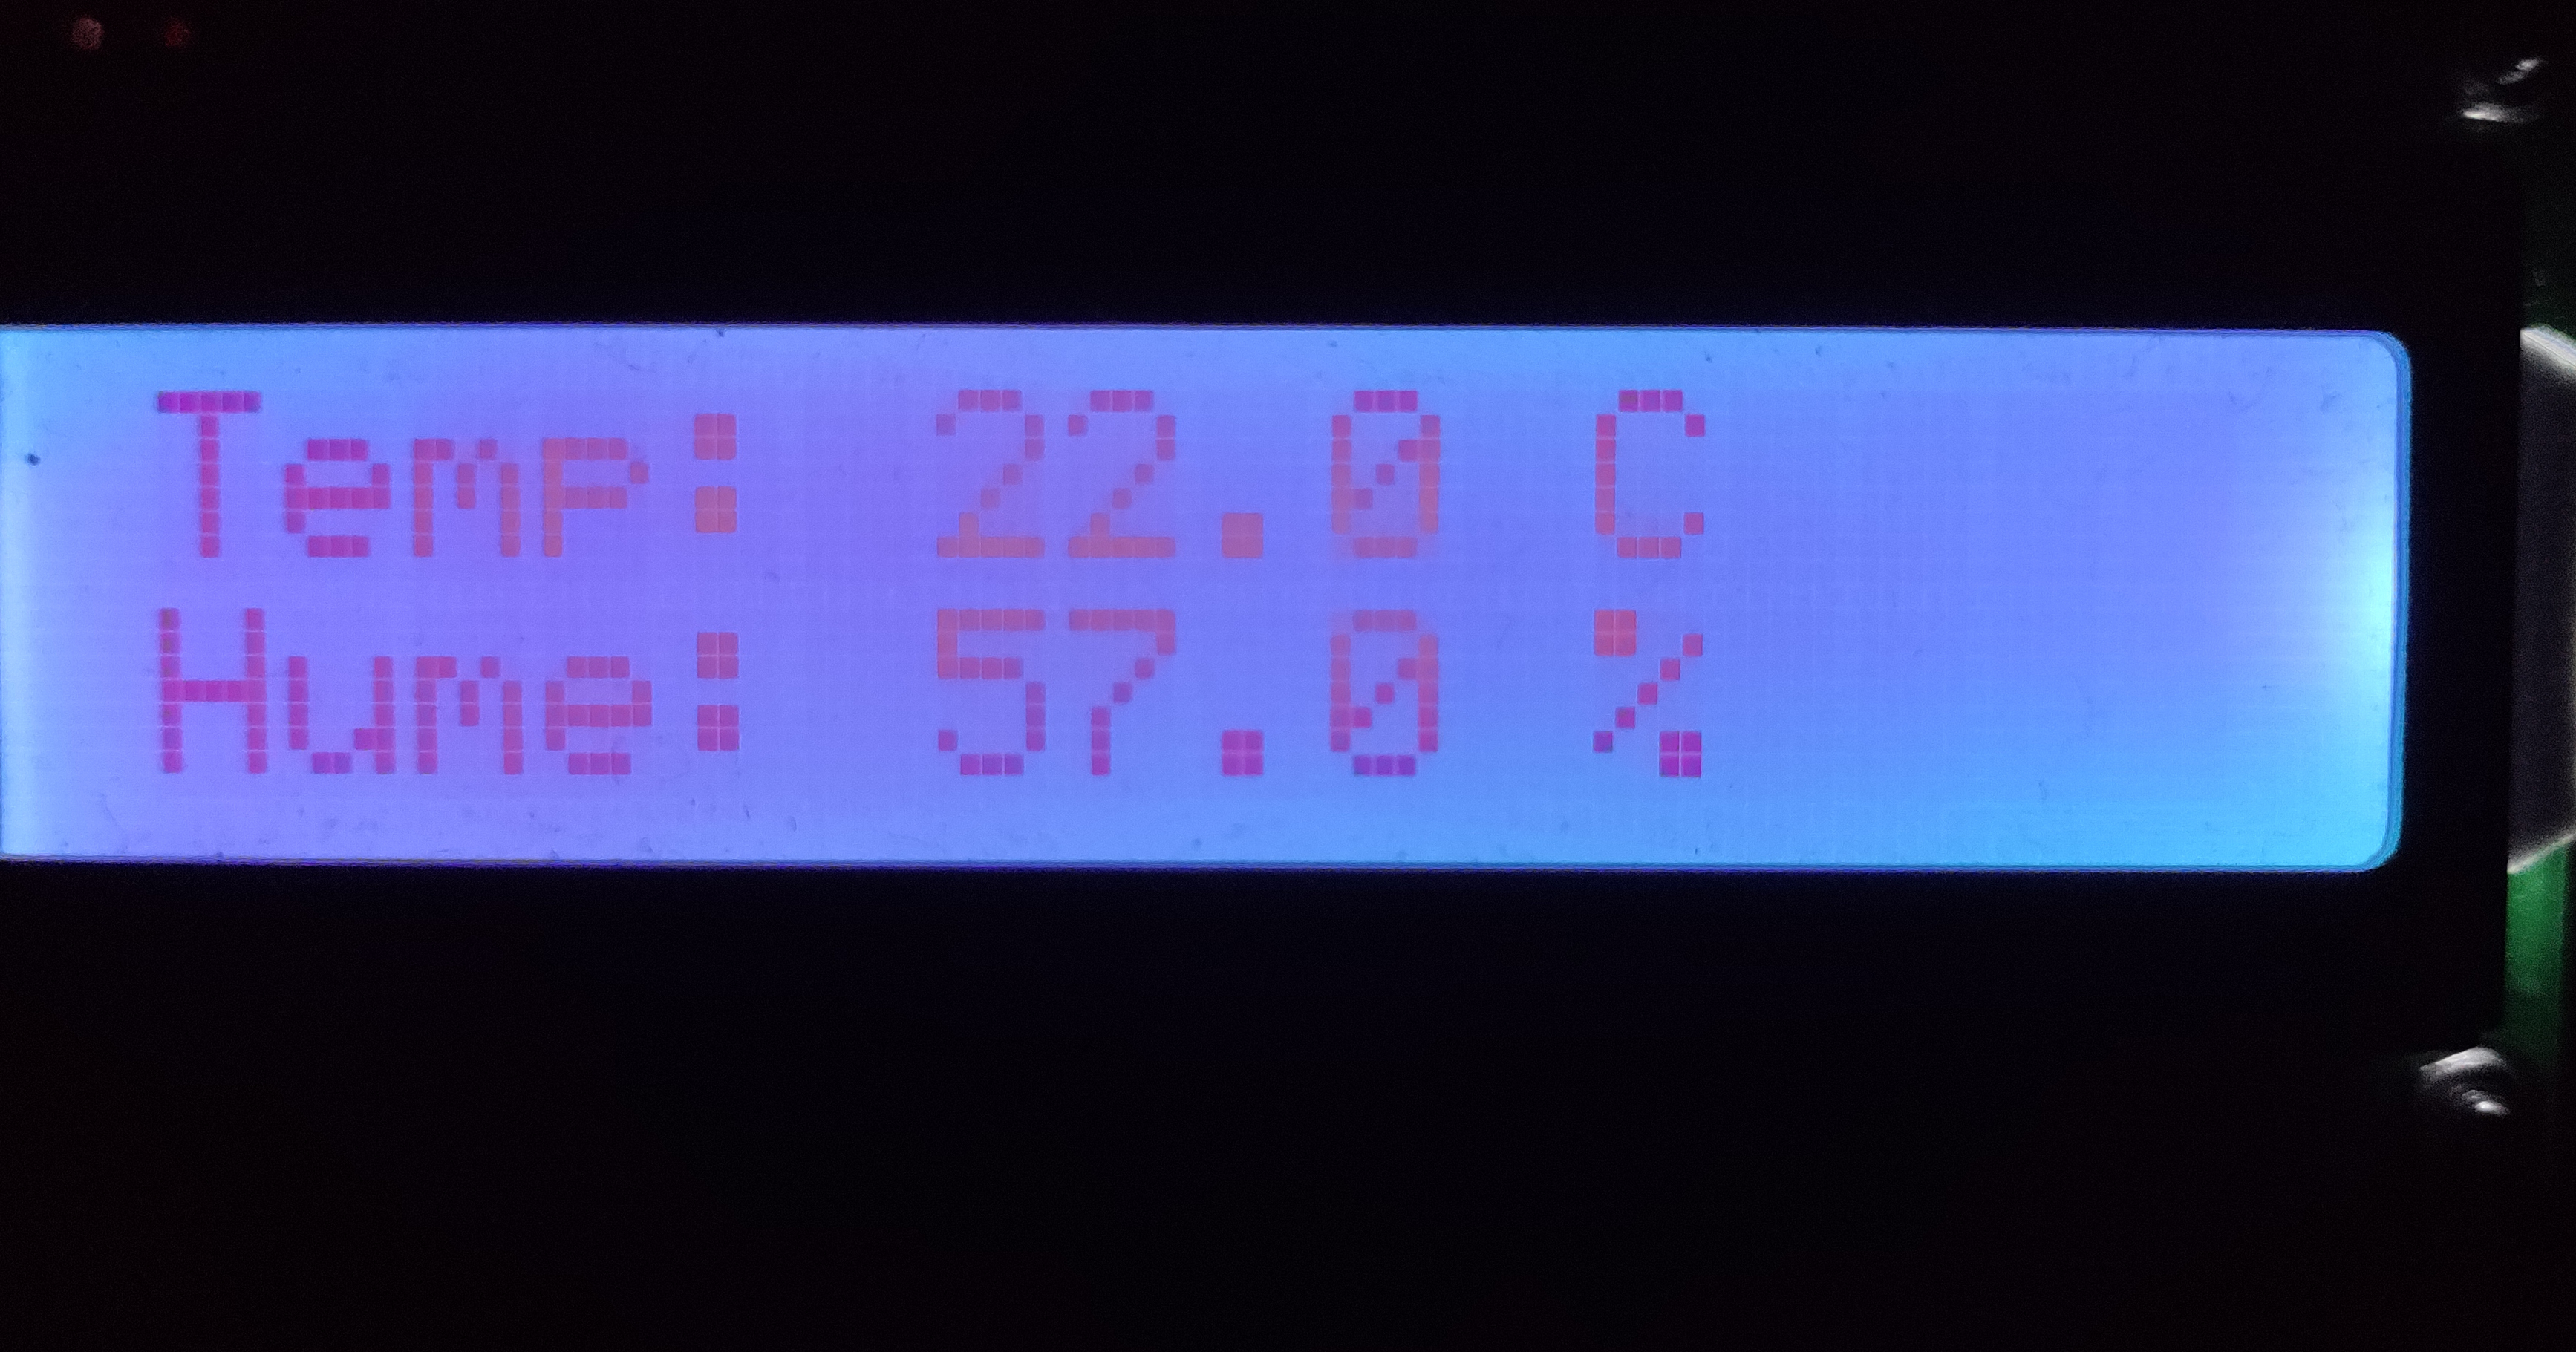
\includegraphics[scale=0.094]{demo_product/DisplayNoche}
  \captionof{figure}{Visualización del display en la oscuridad.}
  \label{fig:DisplayNoche}
\end{center}


En la siguiente sección pueden encontrarse los videos en los que se puede apreciar el funcionamiento del display durante el día \cite{Demo_Mediciones} y en la oscuridad \cite{Demo_Display_Oscuridad}.

\subsection{Prueba y validación del módulo de medición de temperatura y humedad}

Se compararon los valores medidos por el módulo de medición de temperatura y humedad basado en el sensor DHT11 con los obtenidos a través de un dispositivo de medición de temperatura y humedad. Se realizó la medición en diferentes contextos:

\begin{itemize}
	\item En el interior de una casa.
	\item En el exterior, durante el día.
\end{itemize}

En la siguiente tabla se pueden apreciar los resultados.

\begin{table}[h]
\centering
\caption[Resultados de mediciones de temperatura y humedad]{Resultados de mediciones de temperatura y humedad}
\begin{tabular}{l c c c c}
\toprule
\textbf{Contexto} & \textbf{Temp. Robot} & \textbf{Temp. Ref.} & \textbf{Hume. Robot}  & \textbf{Hume. Ref.}\\
\midrule
Interior & 22,0 & 23,6 & 44,0 - 45,0 & 58,5 \\
Exterior (día) & 17,0  & 14,0 & 47,0 - 53,0 & 62,9 - 64,0 \\
Exterior (noche) & - & - & - & - \\
\bottomrule
\hline
\end{tabular}
\end{table}

A continuación, se pueden apreciar algunas fotografías tomadas durante el proceso de experimentación:

\begin{center}
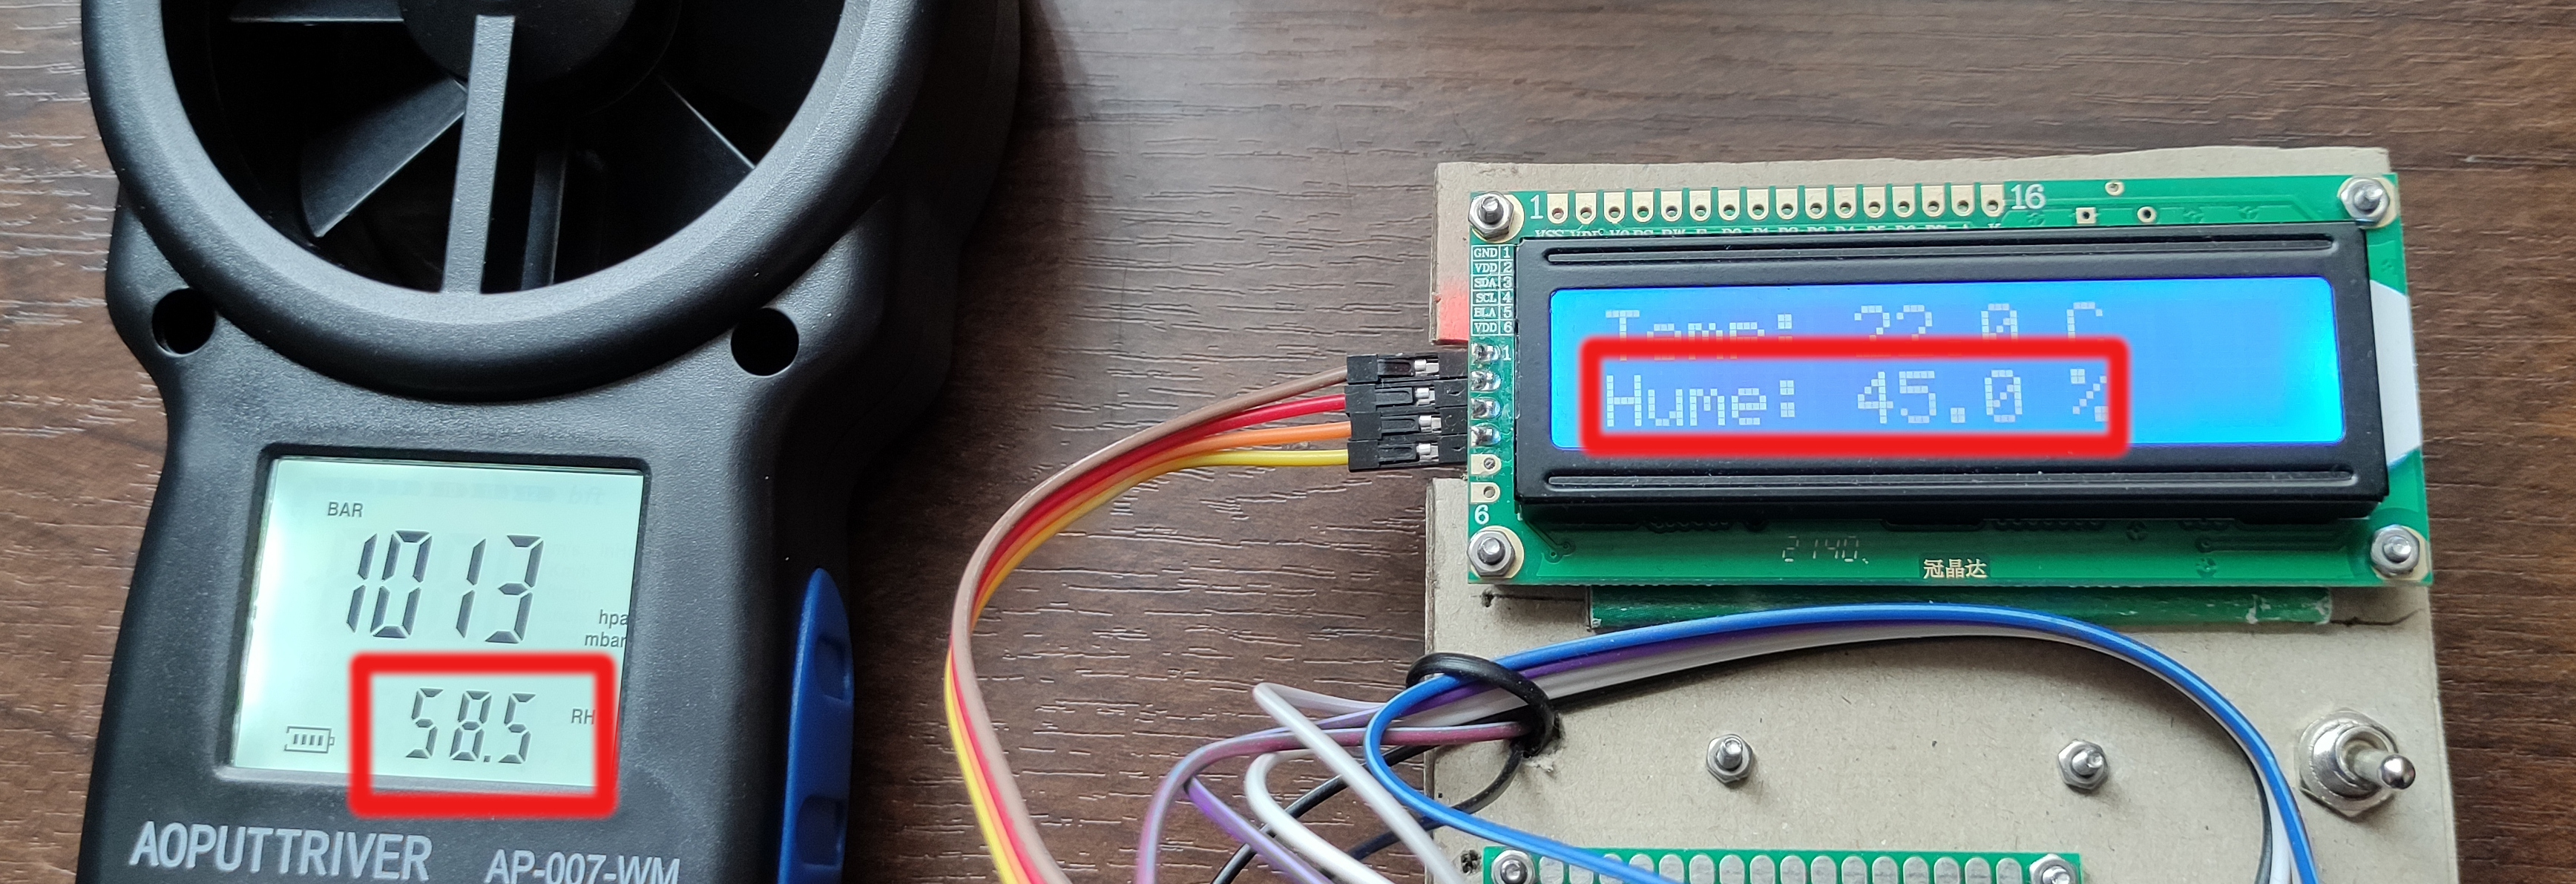
\includegraphics[scale=0.094]{demo_product/humedad_interior_retouched}
  \captionof{figure}{Medición de humedad en el interior.}
  \label{fig:humedad_interior}
\end{center}

\begin{center}
\includegraphics[scale=0.1]{demo_product/temp_interior_retouched}
  \captionof{figure}{Medición de temperatura en el interior.}
  \label{fig:humedad_interior}
\end{center}


\begin{center}
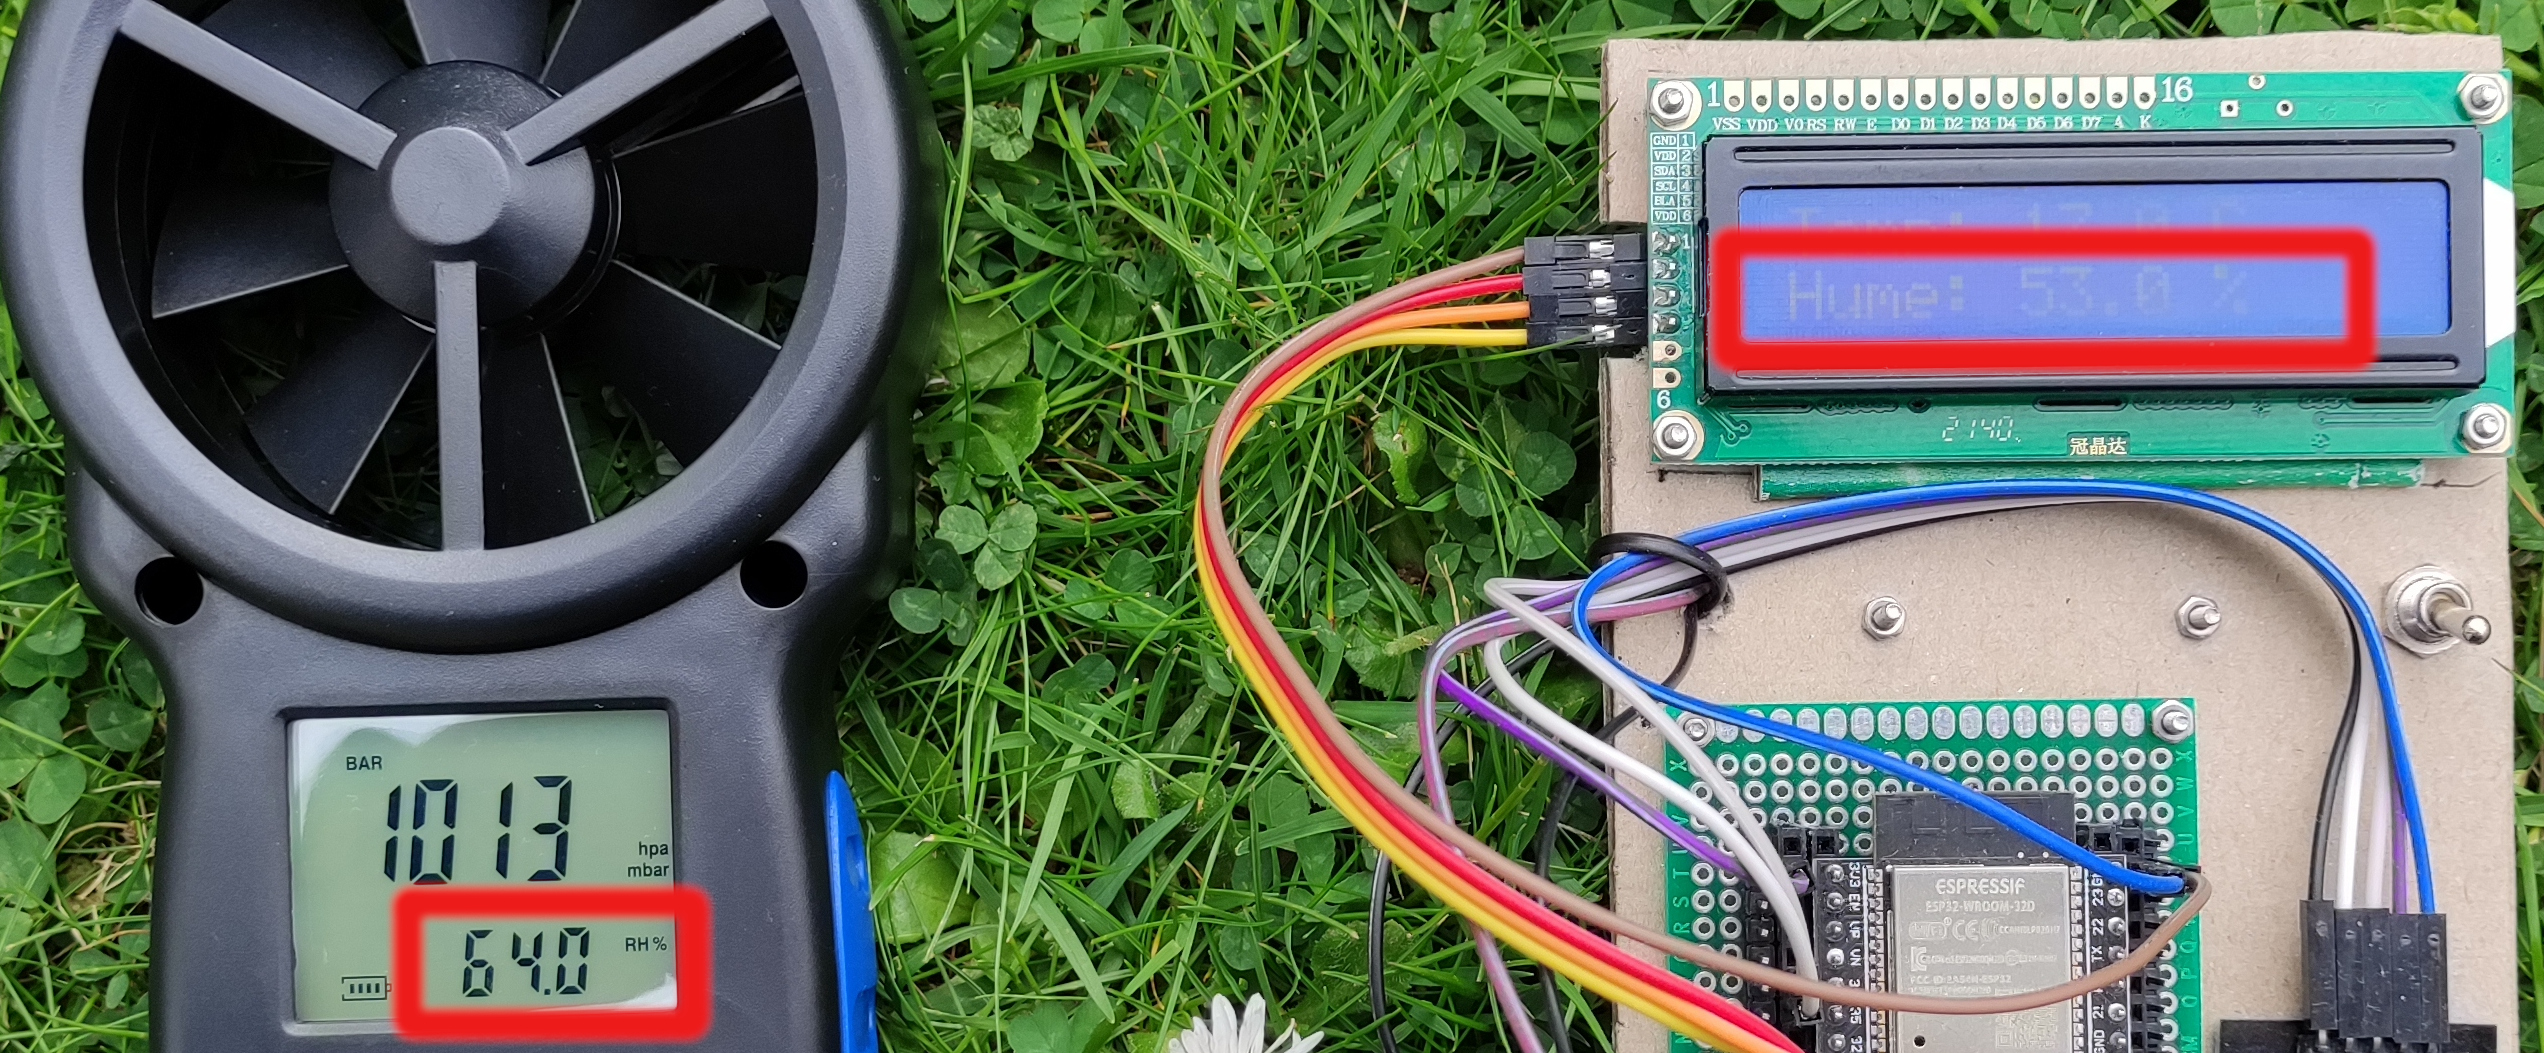
\includegraphics[scale=0.125]{demo_product/humedad_exterior_retouched}
  \captionof{figure}{Medición de humedad en el exterior.}
  \label{fig:humedad_interior}
\end{center}

\begin{center}
\includegraphics[scale=0.1]{demo_product/temp_exterior_dia_retouched}
  \captionof{figure}{Medición de temperatura en el exterior.}
  \label{fig:humedad_interior}
\end{center}

En la siguiente sección puede encontrarse el video que muestra el funcionamiento del módulo de mediciones, en el que se aprecia el funcionamiento del módulo de medición de temperatura y humedad \cite{Demo_Mediciones}.

\subsection{Prueba y validación del módulo de medición de presión atmosférica}

Se compararon los valores medidos por el módulo de medición de presión basado en el sensor BMP280 con los obtenidos a través de un dispositivo manómetro digital. Las mediciones se realizaron en el interior de la vivienda en dos días distintos.

En la siguiente tabla pueden apreciarse los resultados obtenidos:

\begin{table}[h]
\centering
\caption[Resultados de mediciones de presión ambiental.]{Resultados de mediciones de presión ambiental.}
\begin{tabular}{l c c}
\toprule
\textbf{Contexto} & \textbf{Presión. Robot} & \textbf{Presión. Ref.} \\
\midrule
Día 1 & 1013 & 1018,9 \\
Día 2 & 1003,9 & 998 \\
\bottomrule
\hline
\end{tabular}
\end{table}

\begin{center}
\includegraphics[scale=0.1]{demo_product/presion_interior_retouched}
  \captionof{figure}{Medición de presión atmosférica en el interior.}
  \label{fig:humedad_interior}
\end{center}

\begin{center}
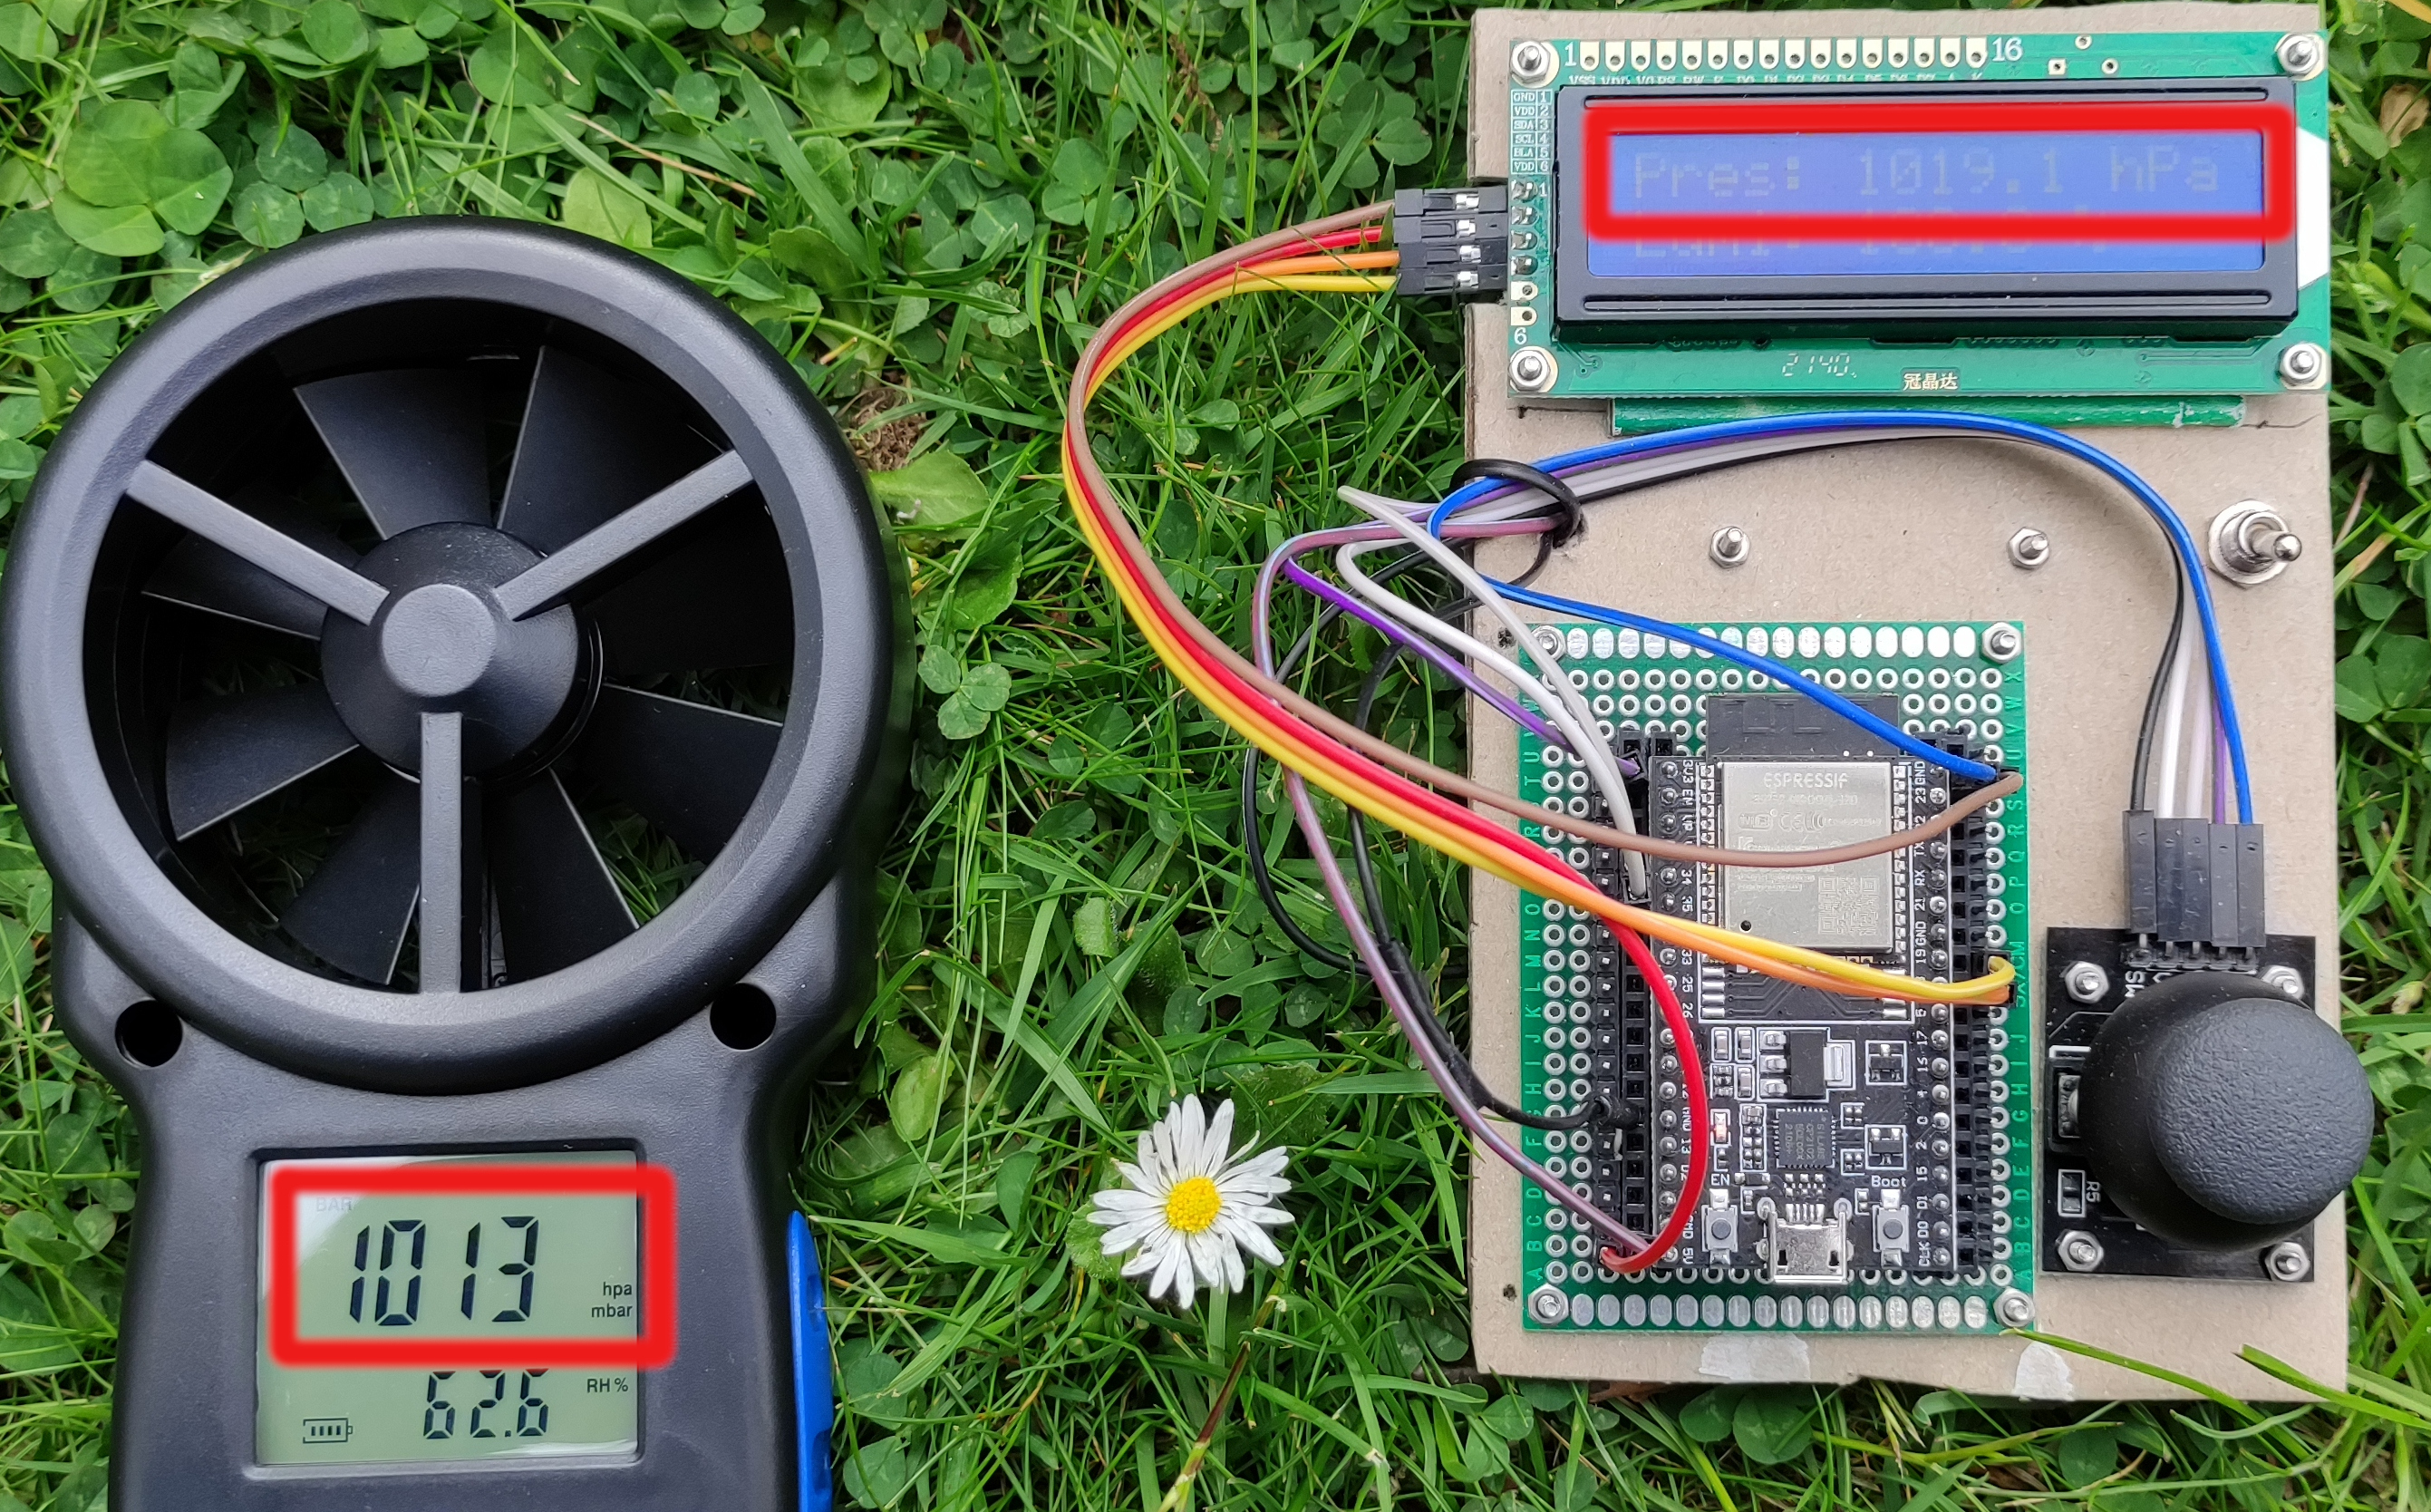
\includegraphics[scale=0.1]{demo_product/presion_exterior_retouched}
  \captionof{figure}{Medición de presión atmosférica en el exterior.}
  \label{fig:humedad_interior}
\end{center}


En la siguiente sección puede encontrarse el video que muestra el funcionamiento del módulo de mediciones, en el que se aprecia el funcionamiento del módulo de medición de presión atmosférica \cite{Demo_Mediciones}.

\subsection{Prueba y validación del módulo de medición de luminosidad ambiental}

Se compararon los valores medidos por el módulo de medición de luminosidad basado en un fotorresistor percibidos por el ojo humano sin utilizar ningún dispositivo de medición. Se realizó la medición en diferentes escenarios:

\begin{itemize}
	\item En exteriores durante el día con luz ambiental.
	\item En interiores con luz ambiental.
	\item En interiores a oscuras.
\end{itemize}

Los resultados mostraron que los valores porcentuales indicados por el módulo de medición de luminosidad son consistentes con los niveles de luz detectados por el ojo humano. En las figuras \ref{fig:DisplayLuminosidadExteriorDia}, \ref{fig:DisplayLuminosidadInteriorDia} y \ref{fig:DisplayLuminosidadInteriorNoche} pueden apreciarse los resultados de las mediciones.

\begin{center}
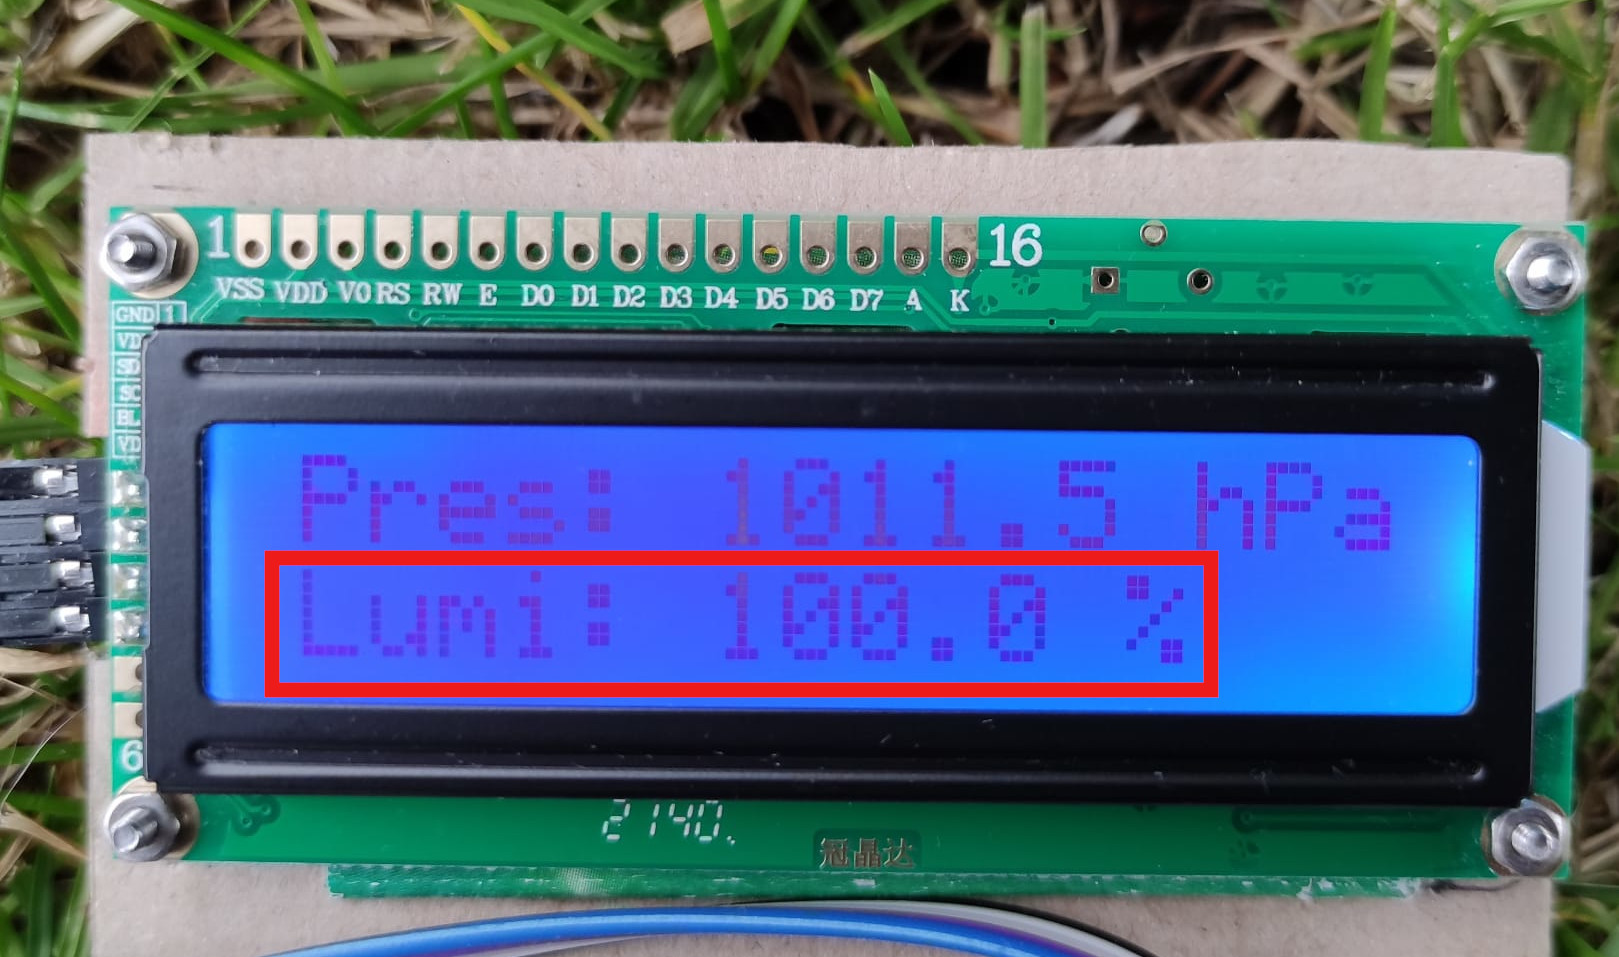
\includegraphics[scale=0.8]{demo_product/DisplayLuminosidadExteriorDia}
  \captionof{figure}{Medición de luminosidad ambiental en el exterior durante el día.}
  \label{fig:DisplayLuminosidadExteriorDia}
\end{center}

\begin{center}
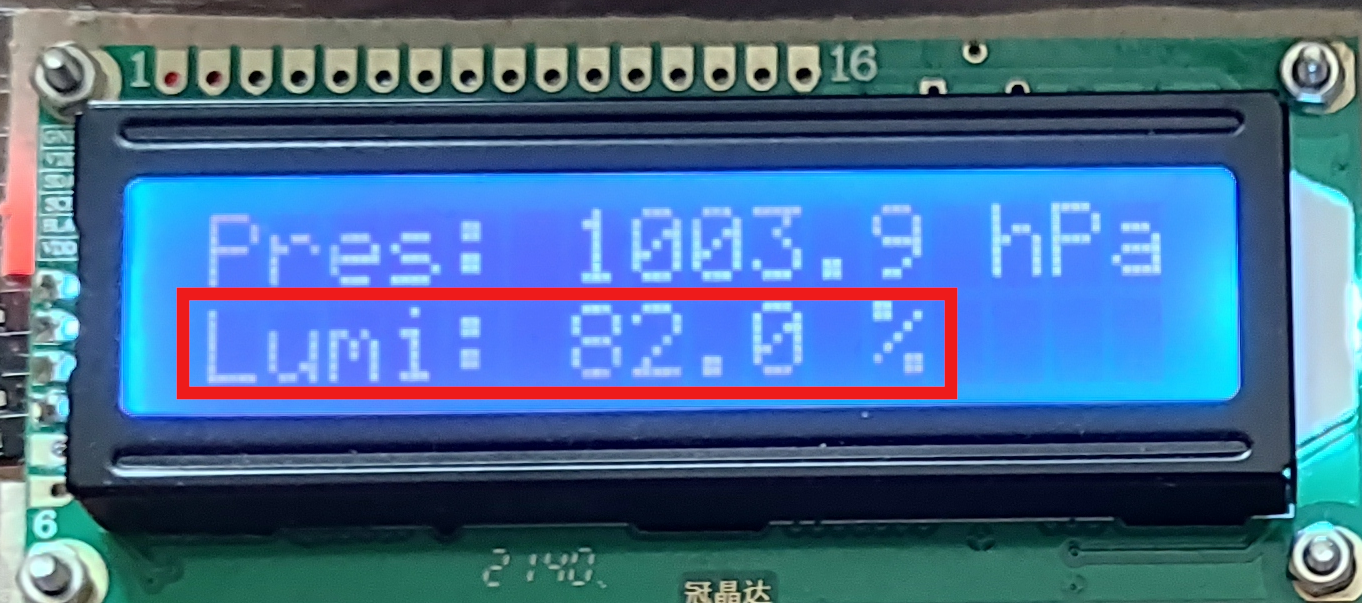
\includegraphics[scale=0.23]{demo_product/DisplayLuminosidadInteriorDia}
  \captionof{figure}{Medición de luminosidad ambiental en interiores durante el día.}
  \label{fig:DisplayLuminosidadInteriorDia}
\end{center}

\begin{center}
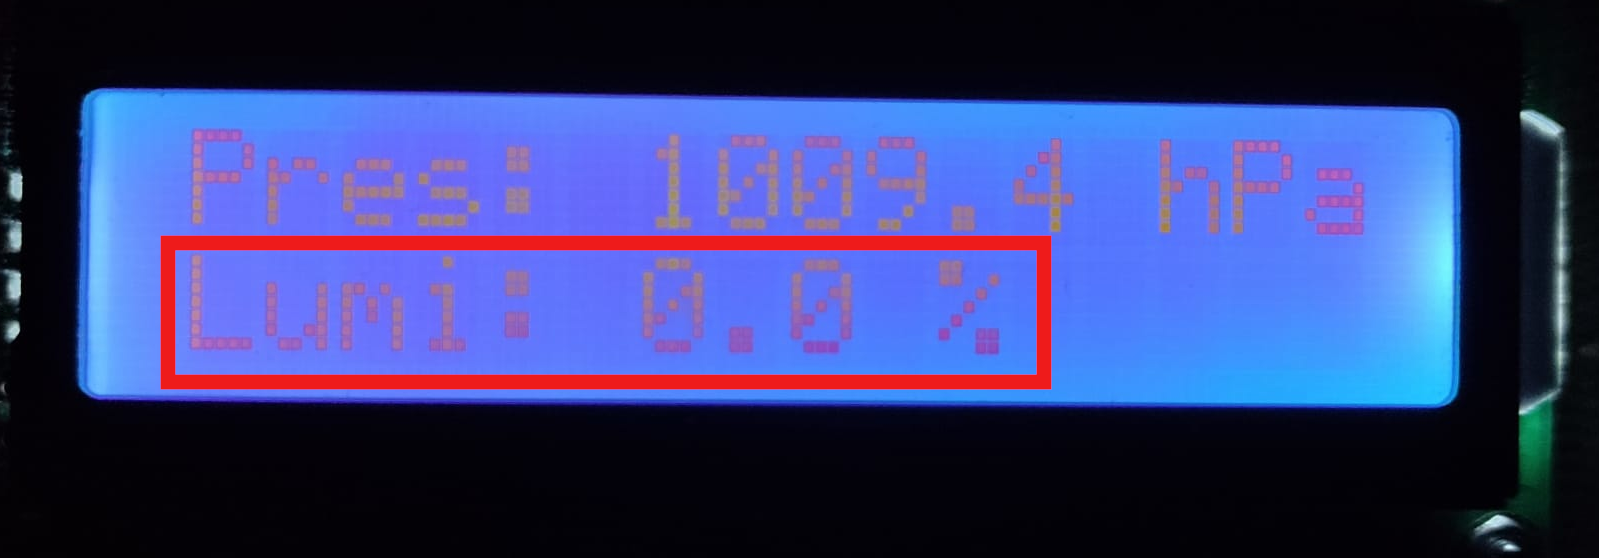
\includegraphics[scale=0.82]{demo_product/DisplayLuminosidadInteriorNoche}
  \captionof{figure}{Medición de luminosidad ambiental en interiores durante la noche.}
  \label{fig:DisplayLuminosidadInteriorNoche}
\end{center}

En la siguiente sección puede encontrarse el video que muestra el funcionamiento del módulo de mediciones, en el que se aprecia el funcionamiento del módulo de medición de luminosidad ambiental \cite{Demo_Mediciones}.

\subsection{Prueba y validación del control y desplazamiento del robot}

Se verificó el control del desplazamiento del robot de forma visual por medio de accionar el joystick en las diferentes coordenadas (X;Y) y se controló que:

\begin{itemize}
	\item La dirección del movimiento del robot sea acorde al accionamiento del joystick.
	\item El tiempo de respuesta en el movimiento del robot y tras el accionar del joystick sea mínimo, permitiendo una buena experiencia de usuario.
\end{itemize}

En la siguiente sección pueden encontrarse los videos \cite{Demo_Control_Movimiento_1} y \cite{Demo_Control_Movimiento_2} evidenciando la demostración de este experimento.



\section{Videos del producto durante el ensamblado y experimentación}

En las siguientes subsecciones se listan los videos realizados durante el proceso de demostración del producto funcionando así como los grabados casualmente durante armado y prototipado del mismo.


\subsection{Videos demostrativos del producto final}

Los experimentos realizados para evidenciar el cumplimiento con los requerimientos funcionales del producto son los siguientes:
\begin{itemize}
	\item Demo - Hardware del producto \cite{Demo_Hardware}.
	\item Demo - Comunicación Wi-Fi \cite{Demo_ComWifi}.
	\item Demo - Control de movimiento de las ruedas \cite{Demo_Control_Movimiento_1}.
	\item Demo - Medición y visualización de parámetros ambientales \cite{Demo_Mediciones}.
	\item Demo - Control de desplazamiento en un circuito \cite{Demo_Control_Movimiento_2}.
	\item Demo - Visualización del Display en la oscuridad \cite{Demo_Display_Oscuridad}.
	
\end{itemize}


\subsection{Videos durante el prototipado y ensamblado del robot}

\begin{itemize}
	\item Prototipado Robot v1 - Ensamblado (1) \cite{Prototipado_Ensamblado_1}.	
	\item Prototipado Robot v1 - Ensamblado (2) \cite{Prototipado_Ensamblado_2}.
	\item Prototipado Robot v1 - Ensamblado (3) \cite{Prototipado_Ensamblado_3}.
	\item Prototipado Robot v1 - Ensamblado (4) \cite{Prototipado_Ensamblado_4}.
	\item Prototipado Robot v2 - Comunicación Joystick Robot (1) \cite{Prototipado_Comunicacion_JoystickRobot1}.
	\item Prototipado Robot v2 - Comunicación Joystick Robot (2) \cite{Prototipado_Comunicacion_JoystickRobot2}.
	\item Prototipado Desplazamiento (alimentación USB) \cite{Prototipado_Desplazamiento_USB}.
	\item Prototipado Desplazamiento (alimentación por pilas) \cite{Prototipado_Desplazamiento_Pilas}.

\end{itemize}




\section{Documentación del producto }

Se desarrolló la documentación del producto compuesta de los siguientes entregables
\begin{itemize}
	\item Documentación técnica \cite{Robot_Tecnical_doc}.
	\item Manual de usuario \cite{Robot_User_manual}.
\end{itemize}











